\documentclass[a4paper,12pt]{Latex/Classes/PhDthesisPSnPDF}
\usepackage[utf8]{inputenc}
\usepackage{amsthm}
\usepackage{graphicx}

% \usepackage[spanish]{babel}
\input{body/preamble/preamble.Rnw}
% This file contains macros that can be called up from connected TeX files
% It helps to summarise repeated code, e.g. figure insertion (see below).

%%%%%%%%%%%%%%%%%%%%%%%%%%%%%%%%%%%%%%%%%%%%%%
%            Colores de la UNAM              %
%%%%%%%%%%%%%%%%%%%%%%%%%%%%%%%%%%%%%%%%%%%%%%
%Azul Pantone 541  -->(0,63,119) RGB
\definecolor{Azul}{RGB}{128,0,0}

%Oro Pantone 460  -->(234,221,150) RGB
\definecolor{Oro}{RGB}{234,221,150}


%%%%%%%%%%%%%%%%%%%%%%%%%%%%%%%%%%%%%%%%%%%%%%
%            Comandos para líneas            %
%%%%%%%%%%%%%%%%%%%%%%%%%%%%%%%%%%%%%%%%%%%%%%
%Se define un comando \colorvrule para hacer líneas verticales de color con 3 argumentos: color, ancho, alto
\newcommand{\colorvrule}[3]{
\begingroup\color{#1}\vrule width#2 height#3
\endgroup}

%Se define un comando \colorhrule para hacer líneas horizontales de color con 2 argumentos: color, ancho
\newcommand{\colorhrule}[2]{
\begingroup\color{#1}\hrule height#2
\endgroup}

%%%%%%%%%%%%%%%%%%%%%%%%%%%%%%%%%%%%%%%%%%%%%%
%          Comando para derivadas            %
%%%%%%%%%%%%%%%%%%%%%%%%%%%%%%%%%%%%%%%%%%%%%%
\newcommand{\derivada}[3][]{\ensuremath{\dfrac{\mbox{d}^{#1}#2}{\mbox{d}#3^{#1}}}} 
%primer argumento(opcional): orden de la derivada
%segundo argumento: función a derivar
%tercer argumento: variable respecto a la que se deriva


%%%%%%%%%%%%%%%%%%%%%%%%%%%%%%%%%%%%%%%%%%%%%%
%       Comando para la exponencial          %
%%%%%%%%%%%%%%%%%%%%%%%%%%%%%%%%%%%%%%%%%%%%%%
\newcommand{\e}[1][]{\ensuremath{\mbox{e}^{#1}}}
%primer argumento(opcional): exponente de la exponencial




% insert a centered figure with caption and description
% parameters 1:filename, 2:title, 3:description and label
\newcommand{\figuremacro}[3]{
	\begin{figure}[htbp]
		\centering
		\includegraphics[width=1\textwidth]{#1}
		\caption[#2]{\textbf{#2} - #3}
		\label{condicion}
	\end{figure}
}

% insert a centered figure with caption and description AND WIDTH
% parameters 1:filename, 2:title, 3:description and label, 4: textwidth
% textwidth 1 means as text, 0.5 means half the width of the text
\newcommand{\figuremacroW}[4]{
	\begin{figure}[htbp]
		\centering
		\includegraphics[width=#4\textwidth]{#1}
		\caption[#2]{\textbf{#2} - #3}
		\label{#1}
	\end{figure}
}

% inserts a figure with wrapped around text; only suitable for NARROW figs
% o is for outside on a double paged document; others: l, r, i(inside)
% text and figure will each be half of the document width
% note: long captions often crash with adjacent content; take care
% in general: above 2 macro produce more reliable layout
\newcommand{\figuremacroN}[3]{
	\begin{wrapfigure}{o}{0.5\textwidth}
		\centering
		\includegraphics[width=0.48\textwidth]{#1}
		\caption[#2]{{\small\textbf{#2} - #3}}
		\label{#1}
	\end{wrapfigure}
}

% predefined commands by Harish
\newcommand{\PdfPsText}[2]{
  \ifpdf
     #1
  \else
     #2
  \fi
}

\newcommand{\IncludeGraphicsH}[3]{
  \PdfPsText{\includegraphics[height=#2]{#1}}{\includegraphics[bb = #3, height=#2]{#1}}
}

\newcommand{\IncludeGraphicsW}[3]{
  \PdfPsText{\includegraphics[width=#2]{#1}}{\includegraphics[bb = #3, width=#2]{#1}}
}

\newcommand{\InsertFig}[3]{
  \begin{figure}[!htbp]
    \begin{center}
      \leavevmode
      #1
      \caption{#2}
      \label{#3}
    \end{center}
  \end{figure}
}







%%% Local Variables:
%%% mode: latex
%%% TeX-master: "~/Documents/LaTeX/CUEDThesisPSnPDF/thesis"
%%% End:
 
\newtheorem{teorema}{Teorema}
\newtheorem{definicion}{Definición}
% \showboxdepth=5
% \showboxbreadth=5
%%%%%%%%%%%%%%%%%%%%%%%%%%%%%%%%%%%%%%%%%%%%%%%%%%%%%%%%%%%%%%%%%%%%%%%%%%%%%%%%
%                                   DATOS                                      %
%%%%%%%%%%%%%%%%%%%%%%%%%%%%%%%%%%%%%%%%%%%%%%%%%%%%%%%%%%%%%%%%%%%%%%%%%%%%%%%%
\title{Evaluación de la Eficacia de una estrategia de trading basada en Modelo Lineal Generalizado}
\author{Rodrigo Alejandro Serrano Morales} 
\facultad{Facultad de Ciencias Económicas y Sociales\\
Escuela de Estadística y Ciencias Actuariales}                % Nombre de la facultad/escuela
\escudofacultad{images/faces} % Aquí ponen la ruta y nombre del escudo de su facultad, actualmente, la carpeta Latex/Classes/Escudos cuenta con los siguientes escudos:
% "fi_azul" Facultad de ingenieria en color azul
% "fi_negro" Facultad de ingenieria en color negro
% "fc_azul" Facultad de ciencias en color azul
% "fc_negro" Facultad de ciencias en color negro
% Se agradecen sus aportaciones de escudos a jebus.velazquez@gmail.com

\degree{Licenciado en Ciencias Actuariales}        % Carrera
\director{Prof. Jonattan Ramos \& Prof. Eloy Eligon}               % Director de tesis
\degreedate{Marzo 2019}                           % Año de la fecha del examen
\lugar{Caracas}                        % Lugar

%\portadafalse                              % Portada en NEGRO, descomentar y comentar la línea siguiente si se quiere utilizar
\portadatrue                                % Portada en COLOR



%% Opciones del posgrado (descomentar si las necesitan)
	%\posgradotrue                                                    
	%\programa{programa de maestría y doctorado en ingeniería}
	%\campo{Ingeniería Eléctrica - Control}
	%% En caso de que haya comité tutor
	%\comitetrue
	%\ctutoruno{Dr. Emmet L. Brown}
	%\ctutordos{Dr. El Doctor}
%% Datos del jurado                             
	%\presidente{Dr. 1}
	%\secretario{Dr. 2}
	%\vocal{Dr. 3}
	%\supuno{Dr. 4}
	%\supdos{Dr. 5}
	%\institucion{el Instituto de Ingeniería, UNAM}

\keywords{tesis,autor,tutor,etc}            % Palablas clave para los metadatos del PDF
\subject{tema_1,tema_2}                     % Tema para metadatos del PDF  

%%%%%%%%%%%%%%%%%%%%%%%%%%%%%%%%%%%%%%%%%%%%%%%%%%%%%
%                   PORTADA                         %
%%%%%%%%%%%%%%%%%%%%%%%%%%%%%%%%%%%%%%%%%%%%%%%%%%%%%
\usepackage{Sweave}
\begin{document}
\Sconcordance{concordance:main.tex:main.Rnw:%
1 64 1 1 0 14 1}
\Sconcordance{concordance:main.tex:./body/introduccion/introduccion.Rnw:ofs 80:%
1 11 1}
\Sconcordance{concordance:main.tex:./body/chapter1/chapter1.Rnw:ofs 92:%
1 43 1}
\Sconcordance{concordance:main.tex:./body/chapter2/chapter2.Rnw:ofs 136:%
1 255 1 1 18 1 2 17 1}
\Sconcordance{concordance:main.tex:./body/chapter3/chapter3.Rnw:ofs 411:%
1 95 1 1 64 3 1 2 2 32 1}
\Sconcordance{concordance:main.tex:./body/chapter4/chapter4.Rnw:ofs 545:%
1 15 1 1 14 3 1 2 2 13 1 1 8 1 3 7 1 1 8 1 2 4 1 1 74 2 1 1 3 1 2 8 1 1 %
3 1 2 8 1 1 3 1 2 8 1 1 12 5 1 1 9 1 2 12 1 1 14 1 2 9 1 1 3 1 2 13 1 1 %
7 1 2 4 1 1 7 3 1 1 7 1 2 22 1 1 3 9 0 1 2 1 1 1 32 1 2 8 0 1 1 7 0 1 2 %
9 0 1 1 10 0 1 2 12 1 1 7 12 0 1 2 3 1 1 6 12 0 1 2 3 1 1 6 12 0 1 2 4 %
1 1 6 12 0 1 2 3 1 1 6 12 0 1 2 4 1 1 6 12 0 1 2 7 1 1 37 2 1 1 2 15 0 %
1 2 3 1 1 26 5 1 1 9 1 2 4 1 1 24 3 1 1 9 1 2 15 1 1 17 2 1 1 2 14 0 1 %
2 3 1 1 27 2 1 1 2 11 0 1 2 2 1}
\Sconcordance{concordance:main.tex:./body/conclusion/conclusion.Rnw:ofs 976:%
1 7 1 1 20 3 1 1 6 1 2 15 1}
\Sconcordance{concordance:main.tex:./body/anexos/anexos.Rnw:ofs 1005:%
1 9 1 1 2 12 0 1 2 3 1 1 2 12 0 1 2 2 1 1 2 12 0 1 2 5 1 1 2 12 0 1 2 3 %
1 1 2 12 0 1 2 2 1 1 2 12 0 1 2 6 1 1 2 12 0 1 2 3 1 1 2 12 0 1 2 3 1 1 %
2 12 0 1 2 5 1 1 2 12 0 1 2 3 1 1 2 12 0 1 2 2 1 1 2 12 0 1 2 6 1 1 2 %
12 0 1 2 3 1 1 2 12 0 1 2 2 1 1 2 12 0 1 2 5 1 1 2 12 0 1 2 3 1 1 2 12 %
0 1 2 2 1 1 2 12 0 1 2 6 1 1 2 12 0 1 2 4 1 1 2 12 0 1 2 2 1 1 2 12 0 1 %
2 5 1 1 2 12 0 1 2 3 1 1 2 12 0 1 2 2 1 1 2 12 0 1 2 1 1}
\Sconcordance{concordance:main.tex:./body/bibliografia/bibliografia.Rnw:ofs 1432:%
1 37 1}
\Sconcordance{concordance:main.tex:main.Rnw:ofs 1470:%
88 1 1}


\maketitle									% Se redefinió este comando en el archivo de la clase para generar automáticamente la portada a partir de los datos

\newpage\renewcommand{\thepage}{\arabic{page}}\setcounter{page}{1} 

% !TeX root = ./main.Rnw
%\SweaveUTF8

\begin{dedication}
Dedicado a mis padres y a mi hermana, por ser los pilares de mi vida y ser mi motivo de haber cumplido esta meta.
\end{dedication}
% !TeX root = ./main.Rnw
%\SweaveUTF8
\newpage
\chapter*{Agradecimientos}

Agradecimientos




  \begin{flushright}
  \textbf{Gracias}
  \end{flushright}

\tableofcontents
\listoffigures
\listoftables


% !TeX root = ./main.Rnw
%\SweaveUTF8

\chapter*{Introducción}
\addcontentsline{toc}{chapter}{Introduccion}

Las economías de países latinoamericanos son reconocidas históricamente por depender en gran magnitud del comercio de sus materias primas, lo cual hace que el comercio con dichos commodities resulte de gran impacto para el gasto fiscal y para la balanza de pagos, esto deja como consecuencia, la necesidad de los actores económicos de estudiar el riesgo a profundidad para poder evitar resultados que reduzcan sus retornos positivos.\\ 

% !TeX root = ./main.Rnw
%\SweaveUTF8

\chapter{El Problema}

\section{Justificación}

El mercado de commodities ha ido evolucionando paralelamente al de otros mercados financieros y actualmente es un mercado globalizado, como el que podemos encontrarnos en los mercados de divisas, de renta variable o de renta fija. Este desarrollo ha permitido la entrada de muchos participantes en el mercado y la implementación de diversos productos e instrumentos de inversión.\\

\section{Planteamiento del Problema}


\section{Objetivo General}

Evaluar la eficacia de una estrategia de trading basada en técnicas de aprendizaje automático en diferentes instrumentos financieros

\section{Objetivos Específicos}

\begin{itemize}
\item Definir los indicadores técnicos a utilizar como variables predictoras
\item Utilizar Análisis de Componentes Principales como técnica de reducción de la dimensión de variables predictoras
\item Aplicar modelo de Regresión Logística con las componentes arrojadas por el ACP
\item Definir la mejor combinación de parametros (Take Profit, Stop Loss y Horizonte) para cada instrumento de inversión según la probabilidad positiva arrojada por el modelo
\item Aplicar el modelo en la data de Validación y analizar resultados
\item Aplicar Montecarlo a la variable ganancia
\end{itemize}

% !TeX root = ./main.Rnw
%\SweaveUTF8

\chapter{Marco Teórico}

\section{Antecedentes}

\subsection{Trading de Cryptomonedas basado en Aprendizaje Automatico}

\subsection{Modelos predictivos para el mercado FOREX}

\subsection{Diseño e implementación de un sistema automatizado para operar en el mercado de divisas usando reglas de asociación}

\section{Bases Teóricas}


\subsection{Hipótesis del Mercado Eficiente}

La Hipótesis del Mercado eficiente fue desarrollada por Eugene Fama en los años 60, en la misma argumenta que los precios de los activos reflejan toda la información disponible, es decir que siempre son transados a un valor adecuado para su riesgo, haciendo imposible para los inversores obtener retornos más elevados que los del mercado en general. 

Fama sugiere tres suposiciones. Primero, el mercado eficiente requiere un gran número de competidores buscando maximizar ganancias. Segundo, la información que afecta al activo llega al mercado de manera aleatoria y cada anuncio es independiente de los demás. Tercero, todos los competirdores intentarán ajustar sus posiciones lo más rapido posible conocida la información del mercado. Existen tres variantes de la hipótesis:

$Eficiencia débil$, en esta variante, los precios del pasado no sirven para predecir el precio futuro, es decir cualquier movimiento del activo es determinado por información no contenida en la serie de precios. $Eficiencia media$, en esta forma se asume que los precios se ajustan instantáneamente a la información pública, por lo que rechaza cualquier tipo de arbitraje intentando aprovechar nueva información. $Eficiencia fuerte$, esta última forma de la hipótesis plantea que los precios reflejan tanto información pública como privada, por lo cual incluso obteniendo información no conocida por todos los competidores, no se pueden obtener retornos anormales a los de los mercados.

Aunque esta hipótesis es la piedra angular de la teoría financiera moderna, es controversial entre la comunidad financiera y dispustada frecuentemente. Algunas de las razones que exponen sus detractores son: 

Los inversores ven la información de manera distinta, por lo que generarán diferentes valuaciones de un mismo activo. Los precios del activo pueden ser afectados por el error humano y desiciones emocionales. Se ha evidenciado en la historia, casos de inversores que han logrado vencer el mercado por largos períodos de tiempo, como Warren Buffet, lo cual por definición de la hipótesis es imposible.

Es evidente la postura que se asume en la presente investigación con respecto a la hipótesis de mercado eficiente. Los avances técnologicos y la capacidad de procesamiento de las computadoras en la actualidad hacen pensar que cualquier anomalía presente en el mercado por muy pequeña que sea puede ser aprovechada por sofisticados softwares automatizados.

\subsection{Análisis Técnico}

Los inversionistas que rechazan la hipótesis del mercado eficiente buscan interpretar la situación del mercado, bien a través de noticias que afecten al activo o estudiando su movimiento intentando extrer patrones de conducta. A la primera técnica se le llama $Análisis Fundamental$ y el segundo $Análisis Técnico$. El Análisis Fundamental está mas asociado a estrategias de inversión pasivas a largo plazo aunque en la actualidad se han desarrollado algoritmos de compra y venta que buscan predecir la dirección del precio en función de noticas utilizando programación Minería de texto.

El análisis técnico es aquel que busca patrones y tendencias de comportamiento en la cotización de los activos financieros, basándose en la serie de tiempo del activo, con esto intenta predecir el movimiento futuro buscando maximizar las ganancias.

%habla del Dow

\subsection{Reglas de asociación}



\subsection{Introducción al aprendizaje automático}

Aprendizaje automático refiere a un amplio abanico de herramientas para el entendimiento de los datos. Estas herramientas pueden ser clasificadas en supervisadas o No Supervisadas

\subsection{Aprendizaje Supervisado y No Supervisado}
\subsection{Métodos de Aprendizaje Supervisado Basado en GLM}
\subsection{Análisis de Componentes Principales como método de reducción de variables}
\subsection{Regresión Logística}
\subsection{Curva ROC}
\subsection{Función de Pérdida}

\section{Bases Legales}


% !TeX root = ./main.Rnw
%\SweaveUTF8

\chapter{Marco Metódico}
\section{Análisis Exploratorio de los datos}

\subsection{Datos OHLC y Fuente de los datos}

La estructura de los datos utilizados en el trabajo es de tipo OHLC por sus siglas en inglés Open, High, Low, Close. La misma, resume en 4 registros el comportamiento del precio del activo (Apertura, Cierre, Mínimo y Máximo) en un intervalo de tiempo. En el caso de la presente investigación, de un día. Este tipo de dato provee la información necesaria para cubrir las exigencia del modelo, tanto para la creación de la variable dependiente como para el cálculo de los indicadores técnicos. 

Los datos fueron extraídos del portal www.investing.com, uno de los portales financieros con mayor prestigio en el mundo. Fue fundado en 2007 y es conocido por su prestigioso calendario económico y directorio de brokers.

\subsection{Series de Índices}

El universo de estudio está representado por los índices bursátiles de los mercados financieros existentes entre el período 26/10/2008 - 18/01/2019. Un índice búrsatil es un promedio de los precios de los activos que representan un mercado o sector determinado. Los mismos sirven como 'benchmark' o referencia de la economía de un país, sector financiero, etc. En el ámbito de los 'hedge funds' son una referencia para medir la rentabilidad de una estrategia de inversión y el riesgo del mercado.

En la presente investigación se utilizan los índices como reflejo del comportamiento de varios activos, de esta manera, se mide la estrategia en un sector y no en un instrumeto en específico. Otras de las ventajas de utilizar los índices es que al representar un promedio de varios activos, sus variaciones son menos drásticas. La muestra está constituida por 5 índices bursátiles que representan distintos mercados del mundo: NASDAQ, NIKKEI, FTSE 100, BOVESPA y SP500.

% hablar de cada indice


\begin{figure}[H]
\setkeys{Gin}{width =0.8\textwidth}
\centering
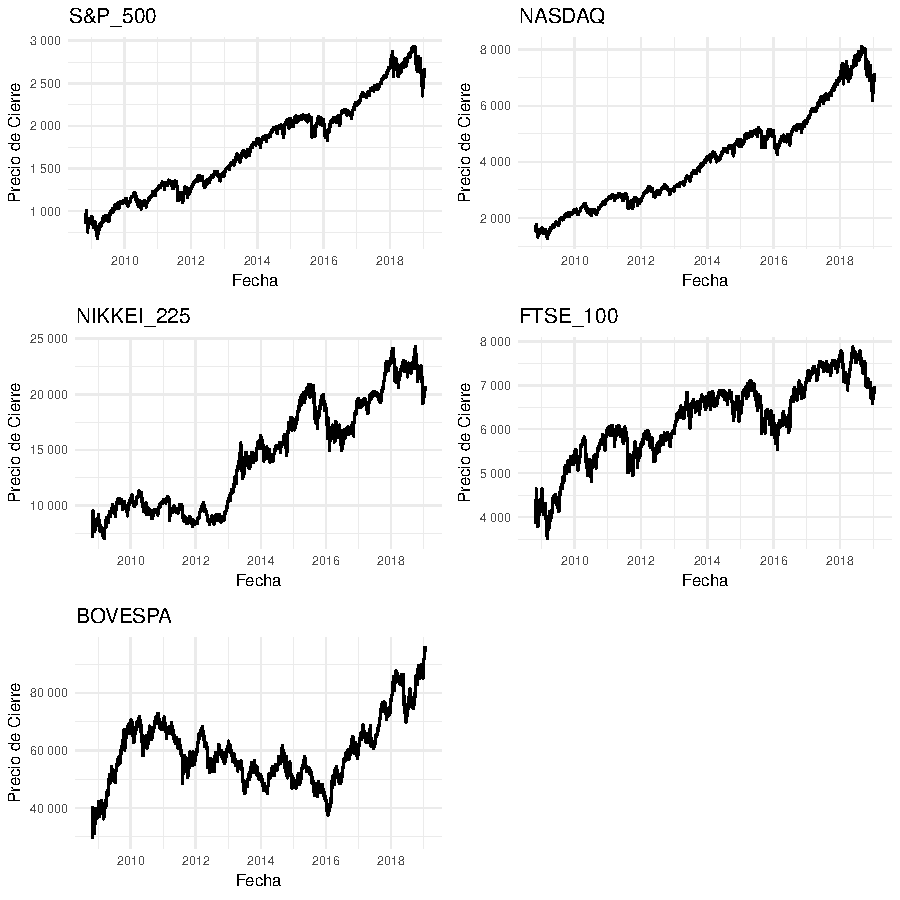
\includegraphics{main-002}
\caption{Precios de Cierre de los índices en el período de estudio (26/10/2008 - 18/01/2019)}
\end{figure}

\section{Entrenamiento del Modelo}

\subsection{Indicadores Técnicos como variables predictoras}

Los indicadores a utilizar fueron seleccionados buscando recoger la mayor información posible sobre el precio del activo que se pueden resumir en tres categorías: tendencia, momentum y volatilidad.

% <!-- Definir las 3 categorías -->

No es de interés en la presente investigación describir como funciona cada indicador para la toma de decisiones en el trading basado en fundamentos técnicos. Cada indicador puede utilizarse de distintas maneras, calcularse con distintos parámetros y asociarse a discreción del trader, lo que conlleva a un sin fin de reglas de asciación. 

Lo que busca la investigación es utilizar la relación entre estos indicadores como variables independientes que ayuden al modelo a predecir oportunidades de entradas. En este sentido se asume la existencia de una dinámica local del mercado que puede ser predecida con ayuda de estos indicadores.

\subsection{Variable dependiente}

Las decisiones de entrada en el trading pueden ser producto de muchos factores, en la presente investigación se analiza el enfoque donde se define un porcentaje objetivo de ganancia y se intenta predecir si dicho objetivo se materializará en un futuro cercano, sin que se haya concretado una venta por Stop Loss. Este enfoque reduce la toma de decisión en una variable tal que:

$$
P_{X}(x) = 
\begin{array}{ll} 
\ \ \ \ p \ ; \qquad x = c
\\
\ 1-p \ ; \qquad x = -d
\end{array}
$$

Dado los datos OHLC del activo es posible identificar los períodos en donde se materializa la variable dependiente. la identificación se realiza, comparando el precio de cierre con los precios máximos y mínimos de las siguientes h observaciones, donde h es el número de períodos, en este caso días en los cuales se desea evaluar la condición.

En la práctica se identifica los registros que cumplen con esta condición añadiendo una columna a la data donde incluimos 'buy' para identificar los registros donde se da la señal y 'stay' en caso de que no haya ocurrido o hubiese ocurrido primero el retroceso del precio.

\subsection{Validación Cruzada en Series de Tiempo}

La validación Cruzada es un metódo de validación y prueba que consiste en dividir los registros aleatoriamente en grupos de similar tamaño. El primer grupo es utilizado como validación del modelo que ha sido entrenado en el resto de los datos, este proceso se realiza k veces, y el resultado final es el promedio arrojado por cada una de las k validaciones.

Ahora bien este método asume que no existe relación entre las observaciones, es decir que son independientes. Esto no es verdad en el caso de las series de tiempo debido a la condicion de autoregresión. Por lo tanto al dividir la data se debe respetar el orden temporal de cada observación. 

\subsection{WalkForward Backtesting}

Al principio de la investigación se implementó el método de entrenamiento, validación y prueba comúnmente utilizado, en donde la mayor parte de la data es destinada a entrenamiento del modelo, otra seccion es destinada a validación, para elegir los parámetros óptimos, y finalmente se testeaba el modelo en la data de prueba. Sin embargo este tipo de metodología en opinión del investigador no es el más óptimo para desarrollar el presente modelo, dado el dinamísmo de los mercados bursátiles la estrategia no puede permanecer estática en el tiempo.

Para contrarestar esta situación se opto por el método de $backtesting Walkforward$, el cual consiste en entrenar el modelo en un período base de data, en este caso los primeros 4 años de estudio, posteriormente se aplica la estrategia en el año siguiente y se obtiene los primeros resultados. Luego este año de aplicación es incluído en la data de entrenamiento -es decir, la data de entrenamiento pasa a ser de 5 años- y se evalúa el modelo en el siguiente año. De esta manera, contemplamos el dinamísmo del mercado permitiendole al modelo -y por ende a la estrategia- utilizar el período mas reciente con respecto al cual será implementado. En la presente figura se ilustra la metodología implementada.

\begin{figure}[ht]
\begin{center}
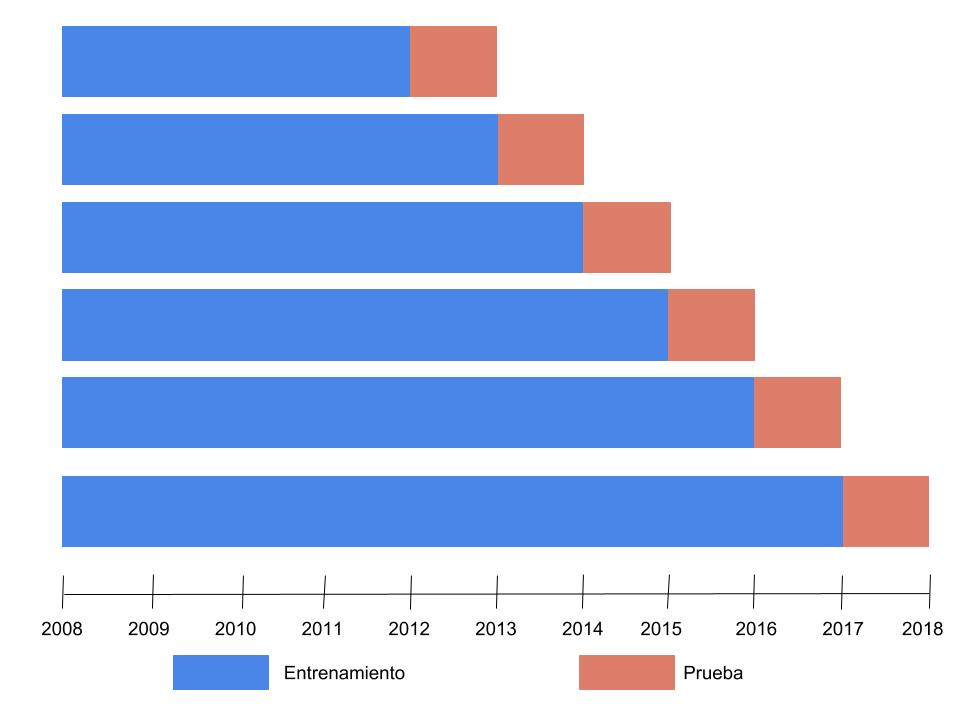
\includegraphics[width=2.5in]{images/walkforward_plot}
\end{center}
\caption{Metodología WalkForward}
\end{figure}

Otra de las caracteristicas de la metodología que se modificó fue la elección de los parámetros óptimos. Previamente se utilizaba la data de validación para buscar la combinación de parámetros óptima. Ahora bien en la metodología de Walkforward se utilizan los mismo parámetros. A opinión del investigador al buscar los mejores parámetros se estaría incurriendo en un posible cesgo de sobreoptimización. El hecho de que en un año determinado unas configuraciones óptimas den los mejores resultados no asegura que se replique en el siguiente año.

La selección de los parámetros debería ser un estudio previo de la serie financiera a testear. En caso de la estrategía actual toma un horizonte de 20 períodos ya que este valor representa un umbral para la ocurrencia del objetivo. Evidentemente al seleccionar un período de tiempo mas corto se obtendrán menos observaciones que cumplan con el patrón por lo tanto estaremos en presencia de un problema de data imbalanceada que debe tener un tratamiento distinto. Por otro lado el utilizar un horizonte mayor no representa gran cambio en el número de ocurrencias, pero sí en el caso de que la transacción quede abierta -hay recordar que h representa una condición de salida para la estrategia, en caso de no ocurrir el target ni el stop loss-.Por lo que se decidió 20 como el número de períodos óptimos a utilizar.


Por su lado el porcentaje de profit se decidió en base a los retornos

\subsection{Reducción de la dimensión con Análisis de Componentes Principales}



\subsection{Evaluación del desempeño del modelo}

En los problemas de clasificación se utiliza la matríz de confusión para evaluar el desempeño del modelo. La misma es una tabla que categoriza las predicciones realizadas por el modelo de acuerdo a la coincidencia con los valores reales. 

\begin{figure}[ht]
\begin{center}
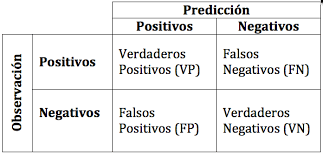
\includegraphics[width=2.5in]{images/confusion_matrix}
\end{center}
\caption{Matríz de Confusión}
\end{figure}

La estrategia solo toma la señal cuando el modelo predice un incremento en el precio, la venta por el contrario no depende del modelo, sino de los parámetros predefinidos (porcentaje de Stop Loss y Horizonte de tiempo). Esta característica implica que el valor a maximizar es la predicción de los verdaderos positivos, conocido como $Precisión$.

$$ Precisión = \frac{VP}{VP + FN} $$

% !TeX root = ./main.Rnw
%\SweaveUTF8

\chapter{Análisis de Resultados}

En el presente capítulo se realiza la descripción de los resultados obtenidos despues de la aplicación del método propuesto para la estrategia. De igual modo, se presentan los resultados arrojados por las pruebas de Backtesting simulando las entradas y salidas.

\section{Series de Rendimientos}

A partir de las series de precios correspondientes a los commodities Petróleo, Oro, Cacao, Harina de Soja y  Aluminio; comprendidas entre el periodo $(10/2010 - 10/2018)$ se calcularon las series de rendimientos logaritmicos para cada uno de los activos. Cabe destacar que se disponen de 1679 observaciones de rendimientos diarios para cada commodity.

\begin{Schunk}
\begin{Sinput}
> list_serie[[1]] %>% head()
\end{Sinput}
\begin{Soutput}
# A tibble: 6 x 5
  timestamp  close  open  high   low
  <date>     <dbl> <dbl> <dbl> <dbl>
1 2008-10-27  849.  874.  894.  847.
2 2008-10-28  941.  849.  941.  845.
3 2008-10-29  930.  940.  970.  922.
4 2008-10-30  954.  939.  963.  928.
5 2008-10-31  969.  953.  984.  945.
6 2008-11-03  966.  969.  976.  959.
\end{Soutput}
\end{Schunk}




% !TeX root = ./main.Rnw
%\SweaveUTF8

\chapter*{Conclusiones y Recomendaciones}
\addcontentsline{toc}{chapter}{Conclusiones y Recomendaciones}

El estudio presentado se centró en confirmar alternativas eficaces para el cálculo del VaR en mercados de materias primas. Los hechos estilizados de las series de tiempo financieras fueron considerados a los largo del trabajo. Y frente a estos planteamientos, se desarrolló una investigación que permitiera detectar una aproximación con el método GARCH-EVT-COPULAS que tuviese la capacidad de estimar el riesgo del mercado de commodities.\\

% !TeX root = ./main.Rnw
%\SweaveUTF8

\chapter*{Lista de Referencias}
\addcontentsline{toc}{chapter}{Lista de Referencias}

\begin{itemize}

\item Alexander, N. Y Zafer, D. (2016). \textit{Gestión del riesgo con el uso de commodities energéticos utilizando Valor en riesgo y Teoría del Valor Extremo}. Suecia, Universidad de Lund.

\end{itemize}

\end{document}
